%%%%%%%%%%%%%%%%%%%%%%%%%%%%%%%%%%%%%%%%%
% Beamer Presentation
% LaTeX Template
% Version 1.0 (10/11/12)
%
% This template has been downloaded from:
% http://www.LaTeXTemplates.com
%
% License:
% CC BY-NC-SA 3.0 (http://creativecommons.org/licenses/by-nc-sa/3.0/)
%
%%%%%%%%%%%%%%%%%%%%%%%%%%%%%%%%%%%%%%%%%
\documentclass[xcolor={table}]{beamer}
\usepackage[utf8]{inputenc}

\mode<presentation> {%

% The Beamer class comes with a number of default slide themes
% which change the colors and layouts of slides. Below this is a list
% of all the themes, uncomment each in turn to see what they look like.

% \usetheme{default}
% \usetheme{AnnArbor}
% \usetheme{Antibes}
% \usetheme{Bergen}
% \usetheme{Berkeley}
% \usetheme{Berlin}
\usetheme{Boadilla}
% \usetheme{CambridgeUS}
% \usetheme{Copenhagen}
% \usetheme{Darmstadt}
% \usetheme{Dresden}
% \usetheme{Frankfurt}
% \usetheme{Goettingen}
% \usetheme{Hannover}
% \usetheme{Ilmenau}
% \usetheme{JuanLesPins}
% \usetheme{Luebeck}
% \usetheme{Madrid}
% \usetheme{Malmoe}
% \usetheme{Marburg}
% \usetheme{Montpellier}
% \usetheme{PaloAlto}
% \usetheme{Pittsburgh}
% \usetheme{Rochester}
% \usetheme{Singapore}
% \usetheme{Szeged}
% \usetheme{Warsaw}

% As well as themes, the Beamer class has a number of color themes
% for any slide theme. Uncomment each of these in turn to see how it
% changes the colors of your current slide theme.

%\usecolortheme{albatross}
%\usecolortheme{beaver}
%\usecolortheme{beetle}
%\usecolortheme{crane}
%\usecolortheme{dolphin}
%\usecolortheme{dove}
%\usecolortheme{fly}
%\usecolortheme{lily}
%\usecolortheme{orchid}
%\usecolortheme{rose}
%\usecolortheme{seagull}
%\usecolortheme{seahorse}
%\usecolortheme{whale}
%\usecolortheme{wolverine}

%\setbeamertemplate{footline} % To remove the footer line in all slides uncomment this line
%\setbeamertemplate{footline}[page number] % To replace the footer line in all slides with a simple slide count uncomment this line

%\setbeamertemplate{navigation symbols}{} % To remove the navigation symbols from the bottom of all slides uncomment this line
}

\usepackage{graphicx} % Allows including images
\usepackage{booktabs} % Allows the use of \toprule, \midrule and \bottomrule in tables
\usepackage{lmodern}%
\usepackage{multicol} % multicols environment
\usepackage{tikz}
\usepackage{amsmath}
\usepackage{amssymb}
\usepackage{textcomp}
\usepackage{pgfplots}
\usepackage{csquotes}
\usepackage{booktabs}                          % Fancy tables
\usepackage[export]{adjustbox}                 % \resizebox
\usepackage{multirow}                          % Fancy tables
\usepackage[table]{xcolor}                     % table option for fancy tables

\definecolor{lightgray}{gray}{0.9}
\definecolor{myeggshell}{RGB}{240,234,214}
\definecolor{mylightgreen}{RGB}{178,255,140}
\definecolor{mylightred}{RGB}{255,161,99}
\usepackage{caption,subcaption} % for tables and figures
\usepgfplotslibrary{groupplots}
\pgfplotsset{compat=1.14}

\pgfdeclarelayer{background}
\pgfsetlayers{background,main}

\usetikzlibrary{arrows,matrix,positioning}
\tikzset{>=latex}
\usetikzlibrary{positioning,calc,fit,chains,arrows}

\usetikzlibrary{positioning,calc,fit,chains,arrows}
\newcommand{\tikzmark}[1]{\tikz[overlay,remember picture] \node (#1) {};}

\usepackage{tikz,overpic}
\usetikzlibrary{fit,shapes.misc}


\newcommand{\thetitle}{Comparing Android Runtime with native:\\Fast Fourier Transform on Android}
\title[Thesis presentation]{\thetitle} % The short title appears at the bottom of every slide, the full title is only on the title page

\author{André Danielsson} % Your name
\institute[KTH] % Your institution as it will appear on the bottom of every slide, may be shorthand to save space
{%
\textit{anddani@kth.se}\\ % Your email address
\medskip
Royal Institute of Technology\\
Computer Science and Communication\\ % Your institution for the title page
}
\date{\today} % Date, can be changed to a custom date

% \AtBeginSection[]
% {%
%   \begin{frame}{~}
%     \makebox[\linewidth][c]{%
%       \begin{minipage}[t][4cm][t]{\textwidth}
%         \begin{multicols}{2}
%           \tableofcontents[currentsection,
%             currentsubsection,
%             subsectionstyle=show/show/shaded,
%           sectionstyle=show/shaded]
%         \end{multicols}
%
%       \end{minipage}%
%     }%
% \end{frame}
% }

\begin{document}

%------------------------------------------------
%	PRESENTATION SLIDES
%------------------------------------------------

% 1.  Present the subject. Describe the work in 1-2 sentences (Intro)
%     (2m)
% 2.  Outline (1m)
% 3.  Why is this important?
%     Where is it used?
%     (1m)
% 4.  Research question
%     (1m)
% 5.  Present the necessary knowledge.
%     Android dev (3m)
%     Vectorization (1m)
%     DFT/FFT (1m)
%     Previous studies (1m)
% 6.  Method
%     Experiments (2m)
%     Measurements (2m)
% 7.  Implementation (2m)
% 8.  Results/Discussion
%     JNI (1m)
%     Libs (1m)
%     NEON (1m)
%     GC (1m)
%     float vs double (1m)
% 9.  Conclusions (1m)
% 10. Questions

% 23

% 262144 256 kB
% 524288 512 kB

%%%------------------------------------------------
%%% Title page, present the work
%%%------------------------------------------------
\begin{frame}
\titlepage%
\end{frame}

%%%------------------------------------------------
%%% Presentation outline
%%%------------------------------------------------
% \begin{frame}{Outline}
%     \makebox[\linewidth][c]{%
%       \begin{minipage}[t][5cm][t]{\textwidth}
%         \begin{multicols}{2}
%           \tableofcontents
%         \end{multicols}
%       \end{minipage}%
%     }%
% \end{frame}

%%%------------------------------------------------
%%% Introduction
%%%------------------------------------------------
\section{Introduction}
%------------------------------------------------
% Purpose of work
%------------------------------------------------
\subsection{Purpose of Thesis}
\begin{frame}{Purpose of Thesis}
    \begin{itemize}
        \item Why is this work important?
        \item Who will benefit from it?
    \end{itemize}
\end{frame}

%------------------------------------------------
% Research Question
%------------------------------------------------
\subsection{Research Question}
\begin{frame}{Research Question}
\centering
\emph{Is there a significant performance difference between implementations of a Fast Fourier Transform (FFT) in native code, compiled by Clang, and Dalvik bytecode, compiled by Android Runtime, on Android?}
\end{frame}

%%%------------------------------------------------
%%% Background
%%%------------------------------------------------
\section{Background}

%------------------------------------------------
% Android
%------------------------------------------------
\subsection{Android Development}
\begin{frame}{Android development}
    \begin{itemize}
        \item<1-> Android Software Development Kit (SDK)
        \item<2-> Android Runtime
        \item<3-> Android Native Development Kit (NDK)
        \item<4-> Java Native Interface (JNI)
    \end{itemize}
\end{frame}
% \begin{frame}{Android SDK}
%     \begin{itemize}
%         \item Framework for developing applications
%         \item Java
%         \item Dalvik Virtual Machine
%     \end{itemize}
% \end{frame}
%
% \begin{frame}{Android Runtime}
%     \begin{itemize}
%         \item Replaced Dalvik Virtual Machine % as default runtime
%         \item Ahead-Of-Time instead of Just-In-Time
%         \item This allows for heavier optimizations
%     \end{itemize}
% \end{frame}
%
% \begin{frame}{Android NDK}
%     \begin{itemize}
%         \item Tools for building native applications
%         \item Uses Clang and LLVM (as of 2017)
%         \item Uses JNI to communicate between Java and Native
%     \end{itemize}
% \end{frame}

%------------------------------------------------
% JNI
%------------------------------------------------
% \subsection{Java Native Interface (JNI)}
% \begin{frame}{Java Native Interface (JNI)}
%     \begin{itemize}
%         \item Bridge between JVM and binaries
%         \item Run code compiled for a specific architecture from Java
%         \item JVM communication
%     \end{itemize}
% \end{frame}


%------------------------------------------------
% Vectorization
%------------------------------------------------
\begin{frame}[t]{Vectorization}
    \begin{center}
    \scalebox{0.7}{%
        \begin{figure}
            \begin{subfigure}{.50\textwidth}
                \centering
                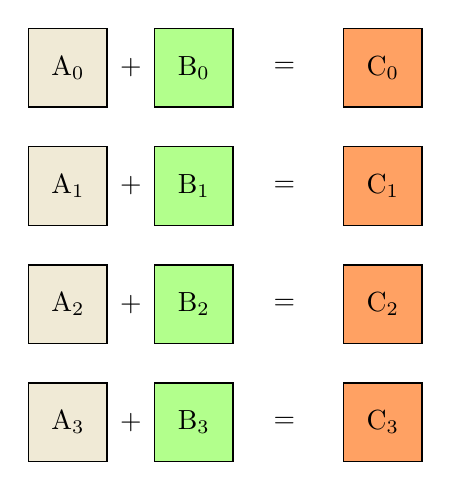
\begin{tikzpicture}[node distance = 0mm, start chain=1 going {below=of \tikzchainprevious.south west}, box/.style = {draw, semithick, minimum size=1cm, every on chain/.style={anchor=north west}, outer sep = 0mm, on chain}]
                    \foreach \i in {1,...,4}
                    {%
                        \pgfmathtruncatemacro{\y}{\i - 1};
                        \pgfmathtruncatemacro{\lab}{(\i - 4) * -1};
                        \node[fill=myeggshell,box] (A\lab) at (0, 1.5*\y) {A$_\lab$};
                        \node[fill=mylightgreen,box] (B\lab) at (1.6, 1.5*\y) {B$_\lab$};
                        \node[fill=mylightred,box] (C\lab) at (4, 1.5*\y) {C$_\lab$};
                        \node[fill=none,right of=A\lab,node distance=0.8cm] (plus\i) {+};
                        \node[fill=none,right of=B\lab,node distance=1.15cm] (equals\i) {=};
                    };
            \end{tikzpicture}%
            \caption{Four separate instructions}
        \end{subfigure}%
        \begin{subfigure}{.50\textwidth}
            \centering
            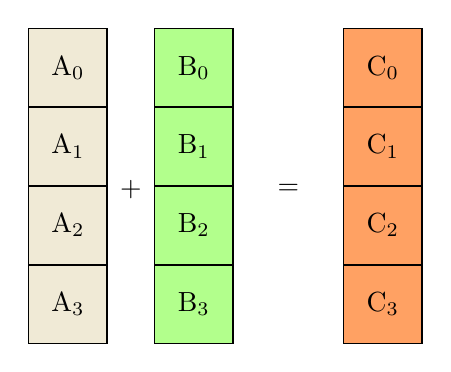
\begin{tikzpicture}[node distance = 0mm, start chain=1 going {below=of \tikzchainprevious.south west}, box/.style = {draw, semithick, minimum size=1cm, every on chain/.style={anchor=north west}, outer sep = 0mm, on chain}]
                \foreach \i in {1,...,4}
                {%
                    \pgfmathtruncatemacro{\y}{\i - 1};
                    \pgfmathtruncatemacro{\lab}{(\i - 4) * -1};
                    \node[fill=myeggshell,box] (A\lab) at (0, 1*\y) {A$_\lab$};
                    \node[fill=mylightgreen,box] (B\lab) at (1.6, 1*\y) {B$_\lab$};
                    \node[fill=mylightred,box] (C\lab) at (4, 1*\y) {C$_\lab$};
                };
            \node[fill=none] (plus) at (1.3, 0.95) {+};
            \node[fill=none] (equals) at (3.3, 0.95) {=};
        \end{tikzpicture}%
        \caption{One instruction with SIMD}
    \end{subfigure}%
    \end{figure}}
    \end{center}
    \begin{itemize}
        \item SSE
        \item NEON
    \end{itemize}
\end{frame}

%------------------------------------------------
% DFT
%------------------------------------------------
\subsection{Discrete Fourier Transform}
\begin{frame}{Discrete Fourier Transform (DFT)}
    \begin{itemize}
        \item DFT: \textit{Time} $\Rightarrow$ \textit{Frequency}
        \item Decomposition of a signal
        \item Example uses:
            \begin{itemize}
                \item Audio visualization
                \item Speech recognition
                \item Compression
            \end{itemize}
        \item Fast Fourier Transform (FFT)
    \end{itemize}

\end{frame}

% \begin{frame}{Discrete Fourier Transform (DFT)}
%     \begin{figure}
    \renewcommand\thesubfigure{(\alph{subfigure})}
    % \centering
    \scalebox{0.7}{%
    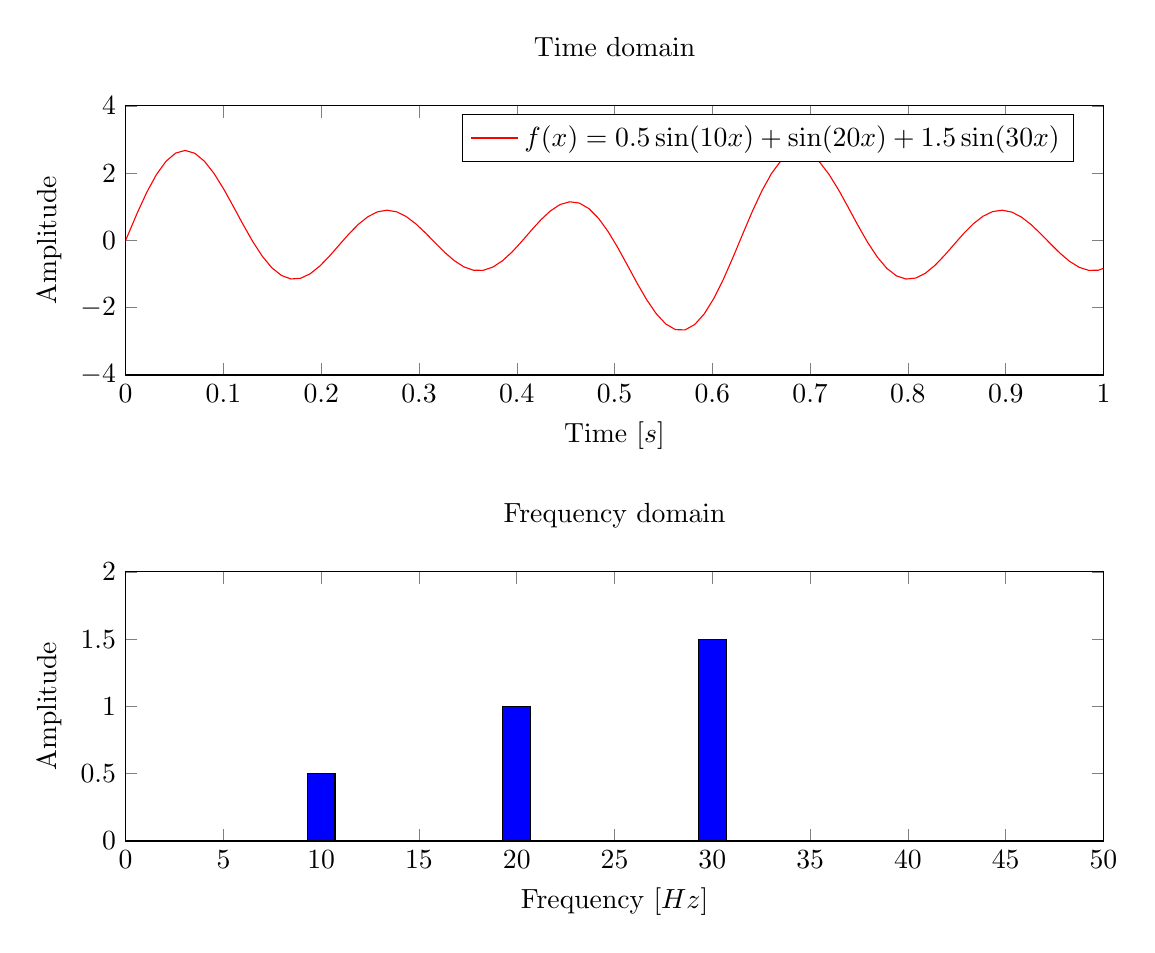
\begin{tikzpicture}
        \begin{groupplot}[group style={group name=my plots,group size= 1 by 2,horizontal sep =1.5cm,vertical sep =2cm},width=6cm]
            \nextgroupplot[
                legend pos=north east,
                trig format plots=rad,
                scaled ticks=false,
                tick label style={/pgf/number format/fixed},
                ymin=-4,
                ymax=4,
                xmin=0,
                xmax=1,
                ylabel={Amplitude},
                xlabel={Time $\left[s\right]$},
                width=14cm,
                height=5cm,
            ]
            \addlegendentry{$f(x) = 0.5\sin(10x) + \sin(20x) + 1.5\sin(30x)$}
            \addplot[domain=-0.5*pi:2*pi,samples=800,red] {0.5*sin(10*x) + sin(20*x) + 1.5*sin(30*x)};
            \nextgroupplot[
                legend pos=north east,
                trig format plots=rad,
                ymin=0,
                ymax=2.0,
                xmin=0,
                xmax=50,
                ylabel={Amplitude},
                xlabel={Frequency $\left[Hz\right]$},
                width=14cm,
                height=5cm,
                yshift=-0.5cm,
            ]
            \addplot[fill=blue,ybar] coordinates {%
                    (10,0.5)
                    (20,1.0)
                    (30,1.5)
                };
            % \addplot[color=blue,mark=none] file {Data/frequencydomain.dat};
        \end{groupplot}
        \node[text width=12cm,align=center,anchor=north] at ([yshift=10mm]my plots c1r1.north) (cap1) {Time domain};
        \node[text width=12cm,align=center,anchor=north] at ([yshift=10mm]my plots c1r2.north) (cap2) {Frequency domain};
    \end{tikzpicture}
    }
\end{figure}

% \end{frame}

%------------------------------------------------
% FFT
%------------------------------------------------
% \begin{frame}{Fast Fourier Transform (FFT)}
%     \begin{itemize}
%         \item Naive DFT, $O(N^2)$:
%             \begin{align*}
%                 X\left(k\right) = \sum\limits_{n=0}^{N-1}x\left(n\right)\cdot e^{-j\frac{2\pi}{N}kn},\ \ k = 0,1,2,\dots,N-1
%             \end{align*}
%         \item Cooley-Tukey FFT\footnote{B. J. W. Cooley and J. W. Tukey, \enquote{An Algorithm for the Machine Calculation Complex Fourier Series}, pp. 297–301, 1964.}, $O(N\log{}N)$
%         \item Trigonometric constants (twiddle factors)
%     \end{itemize}
% \end{frame}
% \begin{frame}{FFT Butterfly updates}
%     \begin{table}
\begin{tabular}{cc}

    \raisebox{-.3\height}{%
        \scalebox{0.7}{%
        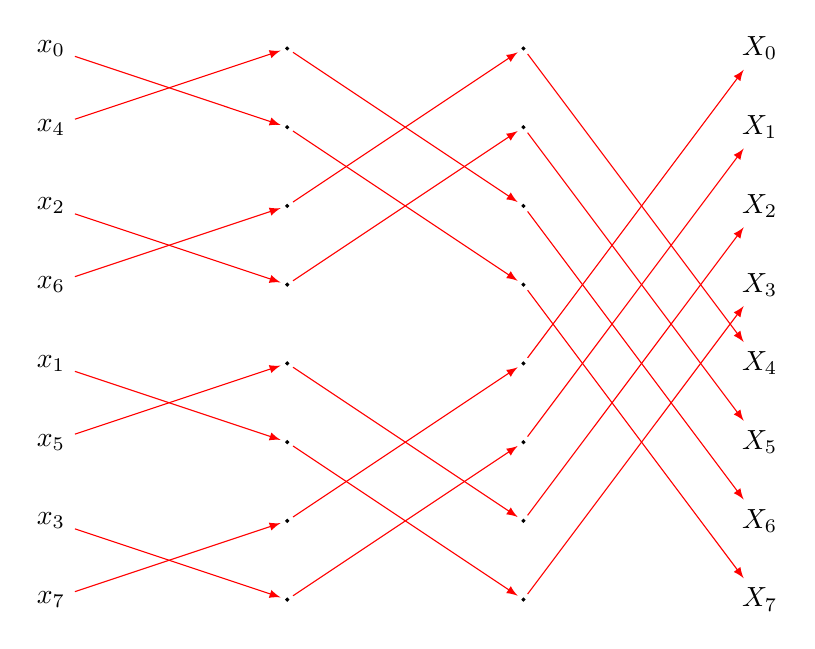
\begin{tikzpicture}[node distance=2cm]
            % nodes
            \node (f0) at (0, 7) {$x_0$};
            \node (f4) at (0, 6) {$x_4$};
            \node (f2) at (0, 5) {$x_2$};
            \node (f6) at (0, 4) {$x_6$};
            \node (f1) at (0, 3) {$x_1$};
            \node (f5) at (0, 2) {$x_5$};
            \node (f3) at (0, 1) {$x_3$};
            \node (f7) at (0, 0) {$x_7$};

            \node [draw,circle,fill=black,inner sep=0pt,outer sep=2pt] (h1) at (3, 7) {};
            \node [draw,circle,fill=black,inner sep=0pt,outer sep=2pt] (h2) at (3, 6) {};
            \node [draw,circle,fill=black,inner sep=0pt,outer sep=2pt] (h3) at (3, 5) {};
            \node [draw,circle,fill=black,inner sep=0pt,outer sep=2pt] (h4) at (3, 4) {};
            \node [draw,circle,fill=black,inner sep=0pt,outer sep=2pt] (h5) at (3, 3) {};
            \node [draw,circle,fill=black,inner sep=0pt,outer sep=2pt] (h6) at (3, 2) {};
            \node [draw,circle,fill=black,inner sep=0pt,outer sep=2pt] (h7) at (3, 1) {};
            \node [draw,circle,fill=black,inner sep=0pt,outer sep=2pt] (h8) at (3, 0) {};

            \node [draw,circle,fill=black,inner sep=0pt,outer sep=2pt] (2h1) at (6, 7) {};
            \node [draw,circle,fill=black,inner sep=0pt,outer sep=2pt] (2h2) at (6, 6) {};
            \node [draw,circle,fill=black,inner sep=0pt,outer sep=2pt] (2h3) at (6, 5) {};
            \node [draw,circle,fill=black,inner sep=0pt,outer sep=2pt] (2h4) at (6, 4) {};
            \node [draw,circle,fill=black,inner sep=0pt,outer sep=2pt] (2h5) at (6, 3) {};
            \node [draw,circle,fill=black,inner sep=0pt,outer sep=2pt] (2h6) at (6, 2) {};
            \node [draw,circle,fill=black,inner sep=0pt,outer sep=2pt] (2h7) at (6, 1) {};
            \node [draw,circle,fill=black,inner sep=0pt,outer sep=2pt] (2h8) at (6, 0) {};

            \node (3h1) at (9, 7) {$X_0$};
            \node (3h2) at (9, 6) {$X_1$};
            \node (3h3) at (9, 5) {$X_2$};
            \node (3h4) at (9, 4) {$X_3$};
            \node (3h5) at (9, 3) {$X_4$};
            \node (3h6) at (9, 2) {$X_5$};
            \node (3h7) at (9, 1) {$X_6$};
            \node (3h8) at (9, 0) {$X_7$};

            % arrows
            % First iteration
            \draw [->,draw=red] (f0) -- (h2);
            \draw [->,draw=red] (f4) -- (h1);
            \draw [->,draw=red] (f2) -- (h4);
            \draw [->,draw=red] (f6) -- (h3);
            \draw [->,draw=red] (f1) -- (h6);
            \draw [->,draw=red] (f5) -- (h5);
            \draw [->,draw=red] (f3) -- (h8);
            \draw [->,draw=red] (f7) -- (h7);

            % Second iteration
            \draw [->,draw=red] (h1) -- (2h3);
            \draw [->,draw=red] (h2) -- (2h4);
            \draw [->,draw=red] (h3) -- (2h1);
            \draw [->,draw=red] (h4) -- (2h2);
            \draw [->,draw=red] (h5) -- (2h7);
            \draw [->,draw=red] (h6) -- (2h8);
            \draw [->,draw=red] (h7) -- (2h5);
            \draw [->,draw=red] (h8) -- (2h6);

            % Third iteration
            \draw [->,draw=red] (2h1) -- (3h5);
            \draw [->,draw=red] (2h2) -- (3h6);
            \draw [->,draw=red] (2h3) -- (3h7);
            \draw [->,draw=red] (2h4) -- (3h8);
            \draw [->,draw=red] (2h5) -- (3h1);
            \draw [->,draw=red] (2h6) -- (3h2);
            \draw [->,draw=red] (2h7) -- (3h3);
            \draw [->,draw=red] (2h8) -- (3h4);
        \end{tikzpicture}
        }%
    }
    &
    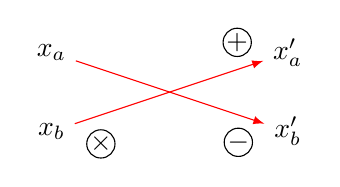
\begin{tikzpicture}[node distance=2cm]

        % nodes
        \node (A) at (0, 0) {$x_b$};
        \node (B) at (0, 1) {$x_a$};
        \node (C) at (3, 0) {$x'_b$};
        \node (D) at (3, 1) {$x'_a$};

        \node [draw,circle,above left=-3mm and 2mm of D,inner sep=0pt] (plus) {$+$};
        \node [draw,circle,below left=-3mm and 2mm of C,inner sep=0pt] (plus) {$-$};
        \node [draw,circle,below right=-2mm and 2mm of A,inner sep=0pt] (plus) {$\times$};

        % arrows
        \draw [->,draw=red] (A) -- (D);
        \draw [->,draw=red] (B) -- (C);

    \end{tikzpicture}
\end{tabular}
\caption*{$x'_a = x_a + x_b\omega^{k}_{N}$\\
          $x'_b = x_a - x_b\omega^{k}_{N}$\\\vspace{0.5mm}
         where $\omega^{k}_{N} = e^{-j\frac{2\pi}{N}}$}
\end{table}

% \end{frame}

%------------------------------------------------
% Related Work
%------------------------------------------------
% \subsection{Related Work}
% \begin{frame}{Related Work}
%     \begin{itemize}
%         \item<1-> S. Lee and J. W. Jeon, \enquote{Evaluating Performance of Android Platform Using Native C for Embedded Systems}, \emph{International Conference on Control, Automation and Systems}, pp. 1160–1163, 2010.
%         \item<2-> A. D. D. C. Jr, M. Rosan, and M. Queiroz, \enquote{FFT benchmark on Android devices: Java versus JNI}, pp. 4–7, 2013.
%         \item<3-> X. Chen and Z. Zong, \enquote{Android App Energy Efficiency: The Impact of Language, Runtime, Compiler, and Implementation}, \emph{2016 IEEE International Conferences on Big Data and Cloud Computing (BDCloud), Social Computing and Networking (SocialCom), Sustainable Computing and Communications (SustainCom)}, pp. 485–492, 2016.
%     \end{itemize}
% \end{frame}

%%%------------------------------------------------
%%% Method
%%%------------------------------------------------
\section{Method}

%------------------------------------------------
% Experiments
%------------------------------------------------
\subsection{Experiments}
\begin{frame}{Experiments}
    \begin{enumerate}
        \item Cost of using JNI
        \item Comparison of smaller FFT libraries
        \item Native optimization with NEON
        % \item Impact of Garbage Collection
        % \item Using \texttt{float} and \texttt{double} data types
    \end{enumerate}
\end{frame}

%------------------------------------------------
% Measurements
%------------------------------------------------
% \subsection{Measurements}
% \begin{frame}{Measurements}
%     \begin{itemize}
%         \item Nexus 6P used in all tests
%         \item Time was measured in Java using \texttt{SystemClock.elapsedRealtimeNanos()}
%         \item Data sizes varied between $2^4 - 2^{18}$
%         \item 100 executions for each test, 95\% confidence interval
%         % \item Garbage collection is a source of error
%     \end{itemize}
% \end{frame}

%------------------------------------------------
% Implementation
%------------------------------------------------
\subsection{Implementation}

\begin{frame}{Implementation}
    \begin{itemize}[<+->]
        \item \textbf{Java}
            \begin{itemize}[<.->]
                \item Princeton Recursive
                \item Princeton Iterative
                \item Columbia Iterative
            \end{itemize}
        \item \textbf{C++}
            \begin{itemize}[<.->]
                \item KISS (Keep It Simple Stupid) FFT
                \item SSE Recursive FFT
                \item SSE Iterative FFT
            \end{itemize}
    \end{itemize}
\end{frame}

\begin{frame}{Implementation}
    \begin{itemize}
        \item Benchmark application
        \item Separate thread, one algorithm at a time
        \item 100 executions, 95\% confidence interval
        % \item Time measurements executed on a release build
    \end{itemize}
\end{frame}

%%%------------------------------------------------
%%% Results and Discussion
%%%------------------------------------------------
\section{Results and Discussion}
\subsection{JNI}
\begin{frame}{JNI (Time \textmu s)}
    \resizebox{\columnwidth}{!}{%
        \rowcolors{1}{}{lightgray}
        \begin{tabular}{lcccc}\toprule
            \textbf{Block size}  & \textbf{No params} & \textbf{Vector} & \textbf{Convert} & \textbf{Columbia}\\\midrule
            \textbf{16}  & 1.7922 $\pm$ 0.1392 & 1.9333 $\pm$ 0.1223 & 2.6052 $\pm$ 0.1004 & 4.1058 $\pm$ 0.3042\\
            \textbf{32}  & 1.6983 $\pm$ 0.0220 & 2.8130 $\pm$ 1.7924 & 2.6006 $\pm$ 0.0370 & 3.9109 $\pm$ 0.0535\\
            \textbf{64}  & 1.6755 $\pm$ 0.0149 & 1.6344 $\pm$ 0.1809 & 2.6630 $\pm$ 0.0425 & 3.9296 $\pm$ 0.0566\\
            \textbf{128}  & 1.9604 $\pm$ 0.4978 & 1.2349 $\pm$ 0.1262 & 1.9375 $\pm$ 0.0843 & 3.0823 $\pm$ 0.0892\\
            \textbf{256}  & 1.7292 $\pm$ 0.0694 & 1.3276 $\pm$ 0.2589 & 1.8141 $\pm$ 0.0276 & 3.0958 $\pm$ 0.0441\\
            \textbf{512}  & 1.6916 $\pm$ 0.0110 & 1.2567 $\pm$ 0.1227 & 2.2818 $\pm$ 0.7011 & 3.1656 $\pm$ 0.0457\\
            \textbf{1024}  & 2.0228 $\pm$ 0.5684 & 1.3167 $\pm$ 0.1341 & \tikzmark{jni1}{6.3756 $\pm$ 8.4676} & 3.2896 $\pm$ 0.1396\\
            \textbf{2048}  & 1.7218 $\pm$ 0.0288 & 1.5416 $\pm$ 0.1405 & 1.9099 $\pm$ 0.0898 & 3.4844 $\pm$ 0.1113\\
            \textbf{4096}  & 1.1411 $\pm$ 0.0404 & 1.4010 $\pm$ 0.0788 & 2.0062 $\pm$ 0.1562 & 3.8562 $\pm$ 0.3197\\
            \textbf{8192}  & 1.1105 $\pm$ 0.0078 & 1.4818 $\pm$ 0.0759 & 2.3671 $\pm$ 0.1897 & 3.8474 $\pm$ 0.4784\\
            \textbf{16384}  & 1.1183 $\pm$ 0.0280 & 1.7308 $\pm$ 0.1043 & 2.5833 $\pm$ 0.1737 & 4.9724 $\pm$ 0.8955\\
            \textbf{32768}  & 1.1162 $\pm$ 0.0084 & 2.2099 $\pm$ 0.1880 & 3.2062 $\pm$ 0.2029 & 5.3719 $\pm$ 0.2875\\
            \textbf{65536}  & 1.7463 $\pm$ 1.2217 & \tikzmark{jni2}{4.7474 $\pm$ 3.1960} & 4.3198 $\pm$ 0.2926 & 6.8136 $\pm$ 0.2499\\
            \textbf{131072}  & 1.1027 $\pm$ 0.0141 & 2.6375 $\pm$ 0.1531 & 5.7004 $\pm$ 0.2681 & 9.6912 $\pm$ 1.4337\\
            \textbf{262144} & 1.1006 $\pm$ 0.0118 & 3.3172 $\pm$ 0.1164 & 7.4630 $\pm$ 0.2309 & 10.2781 $\pm$ 0.2278\\
            \bottomrule
        \end{tabular}
    }
    \pause\tikz[overlay,remember picture]{\draw[draw=red,thick,double,fill opacity=0.2] ($(jni1)+(-1.8,0.3)$) rectangle ($(jni1)+(0.6,-0.1)$);}
    \pause\tikz[overlay,remember picture]{\draw[draw=red,thick,double,fill opacity=0.2] ($(jni2)+(-1.2,0.45)$) rectangle ($(jni2)+(1.2,0.85)$);}
\end{frame}

% \begin{frame}{JNI (Time \textmu s)}
%     \resizebox{\columnwidth}{!}{%
%         \rowcolors{1}{}{lightgray}
%         \begin{tabular}{lcccc}\toprule
%             \textbf{Block size}  & \textbf{No params} & \textbf{Vector} & \textbf{Convert} & \textbf{Columbia}\\\midrule
%             \textbf{16}  & 1.7922 $\pm$ 0.1392 & 1.9333 $\pm$ 0.1223 & 2.6052 $\pm$ 0.1004 & 4.1058 $\pm$ 0.3042\\
%             \textbf{32}  & 1.6983 $\pm$ 0.0220 & 2.8130 $\pm$ 1.7924 & 2.6006 $\pm$ 0.0370 & 3.9109 $\pm$ 0.0535\\
%             \textbf{64}  & 1.6755 $\pm$ 0.0149 & 1.6344 $\pm$ 0.1809 & 2.6630 $\pm$ 0.0425 & 3.9296 $\pm$ 0.0566\\
%             \textbf{128}  & 1.9604 $\pm$ 0.4978 & 1.2349 $\pm$ 0.1262 & 1.9375 $\pm$ 0.0843 & 3.0823 $\pm$ 0.0892\\
%             \textbf{256}  & 1.7292 $\pm$ 0.0694 & 1.3276 $\pm$ 0.2589 & 1.8141 $\pm$ 0.0276 & 3.0958 $\pm$ 0.0441\\
%             \textbf{512}  & 1.6916 $\pm$ 0.0110 & 1.2567 $\pm$ 0.1227 & 2.2818 $\pm$ 0.7011 & 3.1656 $\pm$ 0.0457\\
%             \textbf{1024}  & 2.0228 $\pm$ 0.5684 & 1.3167 $\pm$ 0.1341 & 6.3756 $\pm$ 8.4676 & 3.2896 $\pm$ 0.1396\\
%             \textbf{2048}  & 1.7218 $\pm$ 0.0288 & 1.5416 $\pm$ 0.1405 & 1.9099 $\pm$ 0.0898 & 3.4844 $\pm$ 0.1113\\
%             \textbf{4096}  & 1.1411 $\pm$ 0.0404 & 1.4010 $\pm$ 0.0788 & 2.0062 $\pm$ 0.1562 & 3.8562 $\pm$ 0.3197\\
%             \textbf{8192}  & 1.1105 $\pm$ 0.0078 & 1.4818 $\pm$ 0.0759 & 2.3671 $\pm$ 0.1897 & \tikzmark{jni3}{3.8474 $\pm$ 0.4784}\\
%             \textbf{16384}  & 1.1183 $\pm$ 0.0280 & 1.7308 $\pm$ 0.1043 & 2.5833 $\pm$ 0.1737 & 4.9724 $\pm$ 0.8955\\
%             \textbf{32768}  & 1.1162 $\pm$ 0.0084 & 2.2099 $\pm$ 0.1880 & 3.2062 $\pm$ 0.2029 & 5.3719 $\pm$ 0.2875\\
%             \textbf{65536}  & 1.7463 $\pm$ 1.2217 & 4.7474 $\pm$ 3.1960 & 4.3198 $\pm$ 0.2926 & 6.8136 $\pm$ 0.2499\\
%             \textbf{131072}  & 1.1027 $\pm$ 0.0141 & 2.6375 $\pm$ 0.1531 & 5.7004 $\pm$ 0.2681 & 9.6912 $\pm$ 1.4337\\
%             \textbf{262144} & 1.1006 $\pm$ 0.0118 & 3.3172 $\pm$ 0.1164 & 7.4630 $\pm$ 0.2309 & 10.2781 $\pm$ 0.2278\\
%             \bottomrule
%         \end{tabular}
%     }
%     \tikz[overlay,remember picture]{\draw[draw=red,thick,double,fill opacity=0.2] ($(jni3)+(-2.5,0.6)$) rectangle ($(jni3)+(0.0,-1.8)$);}
% \end{frame}

\begin{frame}{JNI}
    \begin{itemize}
        \item Overhead not significant
        \item JNI implementation differ between VMs
        \item Previous studies have reporter larger execution times
        \item Resolution of Java Timer
    \end{itemize}
\end{frame}

\subsection{Libraries}
\begin{frame}{Libraries (Java)}
    \begin{table}
        \centering
        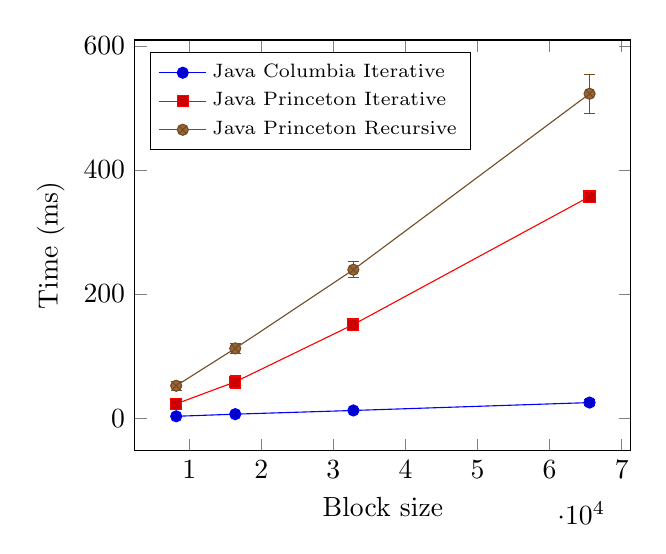
\begin{tikzpicture}
\begin{axis}[xlabel={Block size},ylabel={Time (ms)},width=0.65\linewidth,legend pos=north west,legend cell align=left,legend style={font=\scriptsize}]
\addplot+[error bars/.cd, y dir=both,y explicit] coordinates {
(8192, 2.8726) +- (0.3247, 0.3247)
(16384, 6.3214) +- (1.0542, 1.0542)
(32768, 12.2634) +- (2.9076, 2.9076)
(65536, 24.9874) +- (4.6266, 4.6266)
};
\addplot+[error bars/.cd, y dir=both,y explicit] coordinates {
(8192, 22.9609) +- (5.6248, 5.6248)
(16384, 58.3825) +- (9.9410, 9.9410)
(32768, 150.7299) +- (5.5432, 5.5432)
(65536, 356.9871) +- (8.0942, 8.0942)
};
\addplot+[error bars/.cd, y dir=both,y explicit] coordinates {
(8192, 52.0853) +- (7.1292, 7.1292)
(16384, 112.3024) +- (8.1890, 8.1890)
(32768, 239.0777) +- (12.8962, 12.8962)
(65536, 522.7409) +- (31.4586, 31.4586)
};
\legend{Java Columbia Iterative , Java Princeton Iterative , Java Princeton Recursive}
\end{axis}
\end{tikzpicture}

        \caption{Java line graph for \emph{large} block sizes with standard deviation error bars}
    \end{table}
\end{frame}
\begin{frame}{Libraries (C++)}
    \begin{figure}
        \centering
        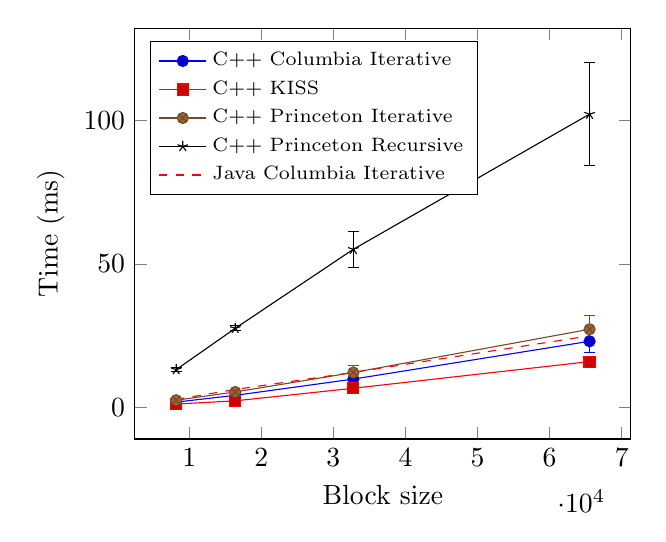
\begin{tikzpicture}
\begin{axis}[xlabel={Block size},ylabel={Time (ms)},width=0.65\linewidth,legend pos=north west,scaled y ticks = false,legend cell align=left,legend style={font=\scriptsize}]
\addplot+[error bars/.cd, y dir=both,y explicit] coordinates {
(8192, 1.9326) +- (0.2654, 0.2654)
(16384, 4.2789) +- (0.6399, 0.6399)
(32768, 9.9388) +- (1.6341, 1.6341)
(65536, 23.1031) +- (3.9019, 3.9019)
};
\addplot+[error bars/.cd, y dir=both,y explicit] coordinates {
(8192, 1.2470) +- (0.2301, 0.2301)
(16384, 2.3713) +- (0.4915, 0.4915)
(32768, 6.7420) +- (1.2931, 1.2931)
(65536, 16.0281) +- (1.8073, 1.8073)
};
\addplot+[error bars/.cd, y dir=both,y explicit] coordinates {
(8192, 2.5845) +- (0.2085, 0.2085)
(16384, 5.4518) +- (0.5858, 0.5858)
(32768, 12.2266) +- (2.4651, 2.4651)
(65536, 27.2805) +- (4.8616, 4.8616)
};
\addplot+[error bars/.cd, y dir=both,y explicit] coordinates {
(8192, 13.2345) +- (0.7311, 0.7311)
(16384, 27.6080) +- (0.9098, 0.9098)
(32768, 55.1227) +- (6.2636, 6.2636)
(65536, 102.1585) +- (17.9911, 17.9911)
};
\addplot+[style=dashed,color=red,mark=none] coordinates {
(8192, 2.8726) +- (0.3247, 0.3247)
(16384, 6.3214) +- (1.0542, 1.0542)
(32768, 12.2634) +- (2.9076, 2.9076)
(65536, 24.9874) +- (4.6266, 4.6266)
};
\legend{C++ Columbia Iterative , C++ KISS , C++ Princeton Iterative , C++ Princeton Recursive, Java Columbia Iterative}
\end{axis}
\end{tikzpicture}

        \caption{C++ line graph for \emph{large} block sizes with standard deviation error bars}
    \end{figure}
\end{frame}
\begin{frame}{Libraries}
    \begin{itemize}
        \item Recursive algorithm worst
        \item Princeton algorithms allocates during run loop
        \item Java Columbia Iterative comparable with C++
        \item Translating Java $\rightarrow$ C++
    \end{itemize}
    % \textbf{problems:} Translating Java $\rightarrow$ C++ may not yield in comparable code. Compilers do different optimizations leading to different execution efficiency. This report is delimited to the chosen compilers and compiler versions.
\end{frame}

\subsection{NEON}
\begin{frame}{NEON}
    \begin{figure}
        \centering
        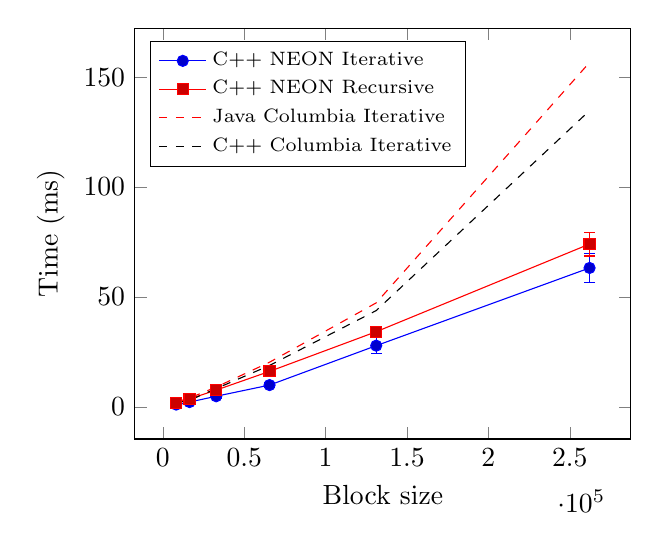
\begin{tikzpicture}
\begin{axis}[xlabel={Block size},ylabel={Time (ms)},width=0.65\linewidth,legend pos=north west,scaled y ticks = false,legend cell align=left,legend style={font=\scriptsize}]
\addplot+[error bars/.cd, y dir=both,y explicit] coordinates {
(8192, 1.0051) +- (0.0657, 0.0657)
(16384, 2.1559) +- (0.2562, 0.2562)
(32768, 4.7898) +- (0.7872, 0.7872)
(65536, 9.8807) +- (1.2509, 1.2509)
(131072, 27.8158) +- (3.6457, 3.6457)
(262144, 63.1858) +- (6.4595, 6.4595)
};
\addplot+[error bars/.cd, y dir=both,y explicit] coordinates {
(8192, 1.6133) +- (0.1416, 0.1416)
(16384, 3.5690) +- (0.4367, 0.4367)
(32768, 7.6009) +- (0.9583, 0.9583)
(65536, 16.1129) +- (1.8936, 1.8936)
(131072, 34.1650) +- (2.4085, 2.4085)
(262144, 74.0746) +- (5.4424, 5.4424)
};
\addplot+[style=dashed,color=red,mark=none] coordinates {
(8192, 2.1766) +- (0.3256, 0.3256)
(16384, 3.9995) +- (0.4596, 0.4596)
(32768, 8.9846) +- (1.3089, 1.3089)
(65536, 20.2833) +- (2.4423, 2.4423)
(131072, 47.2950) +- (6.6700, 6.6700)
(262144, 156.7135) +- (6.0892, 6.0892)
};
\addplot+[style=dashed,color=black,mark=none] coordinates {
(8192, 1.8030) +- (0.9841, 0.9841)
(16384, 2.9629) +- (0.6687, 0.6687)
(32768, 8.2847) +- (1.2061, 1.2061)
(65536, 18.8158) +- (2.8032, 2.8032)
(131072, 43.7807) +- (6.4454, 6.4454)
(262144, 134.8093) +- (10.2633, 10.2633)
};
\legend{C++ NEON Iterative , C++ NEON Recursive, Java Columbia Iterative, C++ Columbia Iterative}
\end{axis}
\end{tikzpicture}

        \caption{NEON results table for \emph{extra large} block sizes, Time (ms)}
    \end{figure}
\end{frame}

\begin{frame}{NEON}
    \begin{itemize}
        \item Vectorization is clearly faster 
        \item Columbia Iterative diverges for larger block sizes
        \item Vectorization tests require some setup
    \end{itemize}
\end{frame}

% \subsection{Garbage Collection}
% \begin{frame}{Garbage Collection}
%     \begin{table}
%         \centering
%         \caption{Pauses due to garbage collection}
%         \resizebox{\columnwidth}{!}{%
%             \rowcolors{1}{}{lightgray}
%             \begin{tabular}{|l|rr|rr|}\toprule
%                 \textbf{Algorithm} & \textbf{\# partial} & \textbf{tot. time (ms)} & \textbf{\# sticky} & \textbf{tot. time (ms)}\\\midrule
%                 \textbf{Java Columbia Iterative}        & 0 & 0 & 0 & 0\\
%                 \tikzmark{gc1}{\textbf{Java Princeton Iterative}} & 477 & 2,825.52 & 406 & 2,959.24\\
%                 \textbf{Java Princeton Recursive}       & 240 & 602.10 & 397 & 887.39\\
%                 \textbf{Java Float Columbia Iterative}  & 0 & 0 & 0 & 0\\
%                 \tikzmark{gc2}{\textbf{Java Float Princeton Iterative}} & 269 & 1,541.97 & 334 & 2,316.53\\
%                 \textbf{Java Float Princeton Recursive} & 167 & 313.05 & 27 & 71.39\\
%                 \textbf{C++ Columbia Iterative}         & 0 & 0 & 0 & 0\\
%                 \textbf{C++ Princeton Iterative}        & 0 & 0 & 0 & 0\\
%                 \textbf{C++ Princeton Recursive}        & 0 & 0 & 0 & 0\\
%                 \textbf{C++ Float Columbia Iterative}   & 0 & 0 & 0 & 0\\
%                 \textbf{C++ Float Princeton Iterative}  & 0 & 0 & 0 & 0\\
%                 \textbf{C++ Float Princeton Recursive}  & 0 & 0 & 0 & 0\\
%                 \textbf{KISS}                           & 0 & 0 & 0 & 0\\
%                 \textbf{NEON Iterative}                 & 0 & 0 & 0 & 0\\
%                 \textbf{NEON Recursive}                 & 0 & 0 & 0 & 0\\
%             \bottomrule
%             \end{tabular}
%         }
%     \end{table}
%     \pause\tikz[overlay,remember picture]{\draw[draw=red,thick,double,fill opacity=0.2] ($(gc1)+(-0.2,-0.4)$) rectangle ($(gc1)+(11.7,-1.1)$);}
%     \tikz[overlay,remember picture]{\draw[draw=red,thick,double,fill opacity=0.2] ($(gc2)+(-0.2,0.0)$) rectangle ($(gc2)+(11.7,-0.7)$);}
% \end{frame}
%
% \begin{frame}[t]{Garbage Collection}
%     % \begin{table}
%         \centering
%         % \caption{Block size where each algorithm started to trigger garbage collection}
%         \resizebox{6cm}{!}{%
%         \rowcolors{1}{}{lightgray}
%         \begin{tabular}{lr}\toprule
%             \textbf{Algorithm} & \textbf{Block Size}\\\midrule
%             \textbf{Princeton Iterative} & 8192\\
%             \textbf{Princeton Recursive} & 4096\\
%             \textbf{Float Princeton Iterative} & 16384\\
%             \textbf{Float Princeton Recursive} & 8192\\
%             \bottomrule
%         \end{tabular}
%         }
%         \vspace{1cm}
%     % \end{table}
%         \begin{itemize}
%             \item Immutable Complex Class
%             \item Many allocations in run loop
%             \item Pre-allocate Arrays to minimize GC
%         \end{itemize}
% \end{frame}
%
% \subsection{\texttt{float} vs \texttt{double}}
% \begin{frame}{\texttt{float} vs \texttt{double}}
%     \begin{table}
%         \centering
%         \caption{Java \texttt{float} results table for \emph{extra large} block sizes, Time (ms)}
%         \resizebox{\columnwidth}{!}{%
%             \rowcolors{1}{}{lightgray}
%             \begin{tabular}{lccc}\toprule
%             \textbf{Block size}  & \textbf{Columbia Iterative} & \textbf{Princeton Iterative} & \textbf{Princeton Recursive}\\\midrule
%             \textbf{32768}  & 8.9846 $\pm$ 0.2566 & 113.1953 $\pm$ 3.9572 & 219.0208 $\pm$ 5.5642\\
%             \textbf{65536}  & 20.2833 $\pm$ 0.4786 & 261.9954 $\pm$ 9.1987 & 485.1020 $\pm$ 13.3737\\
%             \textbf{131072}  & 47.2950 $\pm$ 1.3073 & 622.4328 $\pm$ 24.9022 & 1039.4937 $\pm$ 26.9767\\
%             \tikzmark{ci1}{\textbf{262144}} & 156.7135 $\pm$ 1.1934 & 1728.4640 $\pm$ 53.8042 & 2297.8011 $\pm$ 58.2951\\
%             \bottomrule
%             \end{tabular}
%         }
%     \end{table}
%     \begin{table}
%         \centering
%         \caption{Java \texttt{double} results table for \emph{extra large} block sizes, Time (ms)}
%         \resizebox{\columnwidth}{!}{%
%             \rowcolors{1}{}{lightgray}
%             \begin{tabular}{lccc}\toprule
%             \textbf{Block size}  & \textbf{Columbia Iterative} & \textbf{Princeton Iterative} & \textbf{Princeton Recursive}\\\midrule
%             \textbf{32768}  & 12.2634 $\pm$ 0.5700 & 150.7299 $\pm$ 1.0864 & 239.0777 $\pm$ 2.5276\\
%             \textbf{65536}  & 24.9874 $\pm$ 0.9069 & 356.9871 $\pm$ 1.5864 & 522.7409 $\pm$ 6.1660\\
%             \textbf{131072}  & 85.9483 $\pm$ 1.6097 & 815.8607 $\pm$ 3.4304 & 1144.8802 $\pm$ 17.8736\\
%             \tikzmark{ci2}{\textbf{262144}} & 274.5134 $\pm$ 5.1129 & 2108.0771 $\pm$ 27.5366 & 2638.0547 $\pm$ 40.5424\\
%             \bottomrule
%             \end{tabular}
%         }
%     \end{table}
%     \pause\tikz[overlay,remember picture]{\draw[draw=red,thick,double,fill opacity=0.2] ($(ci1)+(1.9,0.5)$) rectangle ($(ci1)+(4.8,0.0)$);}
%     \tikz[overlay,remember picture]{\draw[draw=red,thick,double,fill opacity=0.2] ($(ci2)+(1.9,0.5)$) rectangle ($(ci2)+(4.8,0.0)$);}
% \end{frame}
%
% \begin{frame}{\texttt{float} vs \texttt{double}}
%     \begin{table}
%         \centering
%         \caption{Java \texttt{float} results table for \emph{extra large} block sizes, Time (ms)}
%         \resizebox{\columnwidth}{!}{%
%             \rowcolors{1}{}{lightgray}
%             \begin{tabular}{lccc}\toprule
%             \textbf{Block size}  & \textbf{Columbia Iterative} & \textbf{Princeton Iterative} & \textbf{Princeton Recursive}\\\midrule
%             \textbf{32768}  & 8.9846 $\pm$ 0.2566 & 113.1953 $\pm$ 3.9572 & 219.0208 $\pm$ 5.5642\\
%             \textbf{65536}  & 20.2833 $\pm$ 0.4786 & 261.9954 $\pm$ 9.1987 & 485.1020 $\pm$ 13.3737\\
%             \textbf{131072}  & 47.2950 $\pm$ 1.3073 & 622.4328 $\pm$ 24.9022 & 1039.4937 $\pm$ 26.9767\\
%             \textbf{262144} & 156.7135 $\pm$ 1.1934 & \tikzmark{pi1}{1728.4640 $\pm$ 53.8042} & 2297.8011 $\pm$ 58.2951\\
%             \bottomrule
%             \end{tabular}
%         }
%     \end{table}
%     \begin{table}
%         \centering
%         \caption{Java \texttt{double} results table for \emph{extra large} block sizes, Time (ms)}
%         \resizebox{\columnwidth}{!}{%
%             \rowcolors{1}{}{lightgray}
%             \begin{tabular}{lccc}\toprule
%             \textbf{Block size}  & \textbf{Columbia Iterative} & \textbf{Princeton Iterative} & \textbf{Princeton Recursive}\\\midrule
%             \textbf{32768}  & 12.2634 $\pm$ 0.5700 & 150.7299 $\pm$ 1.0864 & 239.0777 $\pm$ 2.5276\\
%             \textbf{65536}  & 24.9874 $\pm$ 0.9069 & 356.9871 $\pm$ 1.5864 & 522.7409 $\pm$ 6.1660\\
%             \textbf{131072}  & 85.9483 $\pm$ 1.6097 & 815.8607 $\pm$ 3.4304 & 1144.8802 $\pm$ 17.8736\\
%             \textbf{262144} & 274.5134 $\pm$ 5.1129 & \tikzmark{pi2}{2108.0771 $\pm$ 27.5366} & 2638.0547 $\pm$ 40.5424\\
%             \bottomrule
%             \end{tabular}
%         }
%     \end{table}
%     \tikz[overlay,remember picture]{\draw[draw=red,thick,double,fill opacity=0.2] ($(pi1)+(-0.9,0.5)$) rectangle ($(pi1)+(2.3,0.0)$);}
%     \tikz[overlay,remember picture]{\draw[draw=red,thick,double,fill opacity=0.2] ($(pi2)+(-0.9,0.5)$) rectangle ($(pi2)+(2.3,0.0)$);}
% \end{frame}
%
% \begin{frame}{\texttt{float} vs \texttt{double}}
%     \begin{table}
%         \centering
%         \caption{Java \texttt{float} results table for \emph{extra large} block sizes, Time (ms)}
%         \resizebox{\columnwidth}{!}{%
%             \rowcolors{1}{}{lightgray}
%             \begin{tabular}{lccc}\toprule
%             \textbf{Block size}  & \textbf{Columbia Iterative} & \textbf{Princeton Iterative} & \textbf{Princeton Recursive}\\\midrule
%             \textbf{32768}  & 8.9846 $\pm$ 0.2566 & 113.1953 $\pm$ 3.9572 & 219.0208 $\pm$ 5.5642\\
%             \textbf{65536}  & 20.2833 $\pm$ 0.4786 & 261.9954 $\pm$ 9.1987 & 485.1020 $\pm$ 13.3737\\
%             \textbf{131072}  & 47.2950 $\pm$ 1.3073 & 622.4328 $\pm$ 24.9022 & 1039.4937 $\pm$ 26.9767\\
%             \textbf{262144} & 156.7135 $\pm$ 1.1934 & 1728.4640 $\pm$ 53.8042 & \tikzmark{pr1}{2297.8011 $\pm$ 58.2951}\\
%             \bottomrule
%             \end{tabular}
%         }
%     \end{table}
%     \begin{table}
%         \centering
%         \caption{Java \texttt{double} results table for \emph{extra large} block sizes, Time (ms)}
%         \resizebox{\columnwidth}{!}{%
%             \rowcolors{1}{}{lightgray}
%             \begin{tabular}{lccc}\toprule
%             \textbf{Block size}  & \textbf{Columbia Iterative} & \textbf{Princeton Iterative} & \textbf{Princeton Recursive}\\\midrule
%             \textbf{32768}  & 12.2634 $\pm$ 0.5700 & 150.7299 $\pm$ 1.0864 & 239.0777 $\pm$ 2.5276\\
%             \textbf{65536}  & 24.9874 $\pm$ 0.9069 & 356.9871 $\pm$ 1.5864 & 522.7409 $\pm$ 6.1660\\
%             \textbf{131072}  & 85.9483 $\pm$ 1.6097 & 815.8607 $\pm$ 3.4304 & 1144.8802 $\pm$ 17.8736\\
%             \textbf{262144} & 274.5134 $\pm$ 5.1129 & 2108.0771 $\pm$ 27.5366 & \tikzmark{pr2}{2638.0547 $\pm$ 40.5424}\\
%             \bottomrule
%             \end{tabular}
%         }
%     \end{table}
%     \tikz[overlay,remember picture]{\draw[draw=red,thick,double,fill opacity=0.2] ($(pr1)+(-1.4,0.5)$) rectangle ($(pr1)+(2.0,0.0)$);}
%     \tikz[overlay,remember picture]{\draw[draw=red,thick,double,fill opacity=0.2] ($(pr2)+(-1.4,0.5)$) rectangle ($(pr2)+(2.0,0.0)$);}
% \end{frame}
%
% \begin{frame}{\texttt{float} vs \texttt{double}}
%     \begin{itemize}
%         \item Likely due to caching
%         \item \texttt{float} $\rightarrow$ 32-bit
%         \item \texttt{double} $\rightarrow$ 64-bit
%     \end{itemize}
% \end{frame}


%%%------------------------------------------------
%%% Conclusions
%%%------------------------------------------------
\section{Conclusions}
\begin{frame}{Conclusions}
    \begin{block}{Conclusion 1}
        \emph{The overhead from JNI does not have a significant effect on performance.}
    \end{block}
    \begin{block}{Conclusion 2}
        \emph{Of the tested algorithms, choose Columbia Iterative.}
    \end{block}
    \begin{block}{Conclusion 3}
        \emph{Avoid allocating memory in the run-loop of a recurring task.}
    \end{block}
    \begin{block}{Conclusion 4}
        \emph{NEON optimization is significantly faster than non-optimized code for larger block sizes.} % Mention image processing, more data
    \end{block}
\end{frame}

\begin{frame}
    \Huge{\centerline{Questions?}}
\end{frame}

\end{document}
